%\section{Models and parameter estimation}
%\input Sections/model_Nancy.tex

In this section we first remind the reader of the definition of a hidden Markov model (HMM). We then review three variations on the HMM; the CarHMM, HHMM, and HMM-DFT. Finally, we generalize the hierarchical structure of these models and describe how they can be flexibly altered and combined to form new models.

%%%%%%%%%%%%%%%%%%%%%%%%%%%%%%%%%%%%%%%%%
\subsection{The hidden Markov model (HMM)}

A \textit{hidden Markov model}  is comprised of a sequence of  unobserved states $X_t$, $t = 1, \ldots, T$, and an associated sequence of  possibly high-dimensional observations $Y_t$, $t = 1, \ldots, T$,
The $Y_t$s are often referred to as ``emissions'' and the index $t$ typically refers to time. 
The $X_t$s form a Markov chain and take possible values $1, \ldots, N$. Their distribution is governed by the distribution of the initial state $X_1$ and the $N \times N$ transition probability matrix $\Gamma$ where $\Gamma_{ij} = \Pr(X_{t+1} = j | X_t = i)$, for $t=1,\ldots, T-1$, and $i, j = 1,\ldots, N$. 
%
We assume that $X_1$ follows the chain's stationary distribution, which is denoted by $\delta \in \bbR^N$, with $i$th component
$\delta_i = \Pr\{X_1 = i\},~ i = 1,\ldots,N.$
%
Recall that a Markov chain's stationary distribution is determined by its probability transition matrix via $\delta = \delta \Gamma$ and $\sum_{i=1}^N \delta_i = 1$.
%
The distribution of an emission $Y_t$ depends only on the corresponding state $X_t$ and no other observations or hidden states: $p\left(y_t|\{X_1,\ldots, X_T\},\{Y_1,\ldots, Y_T\}/ \{Y_t\}\right) = p(y_t|X_t)$.
%
These conditional distributions are governed by state-dependent parameters: if $X_t = i$, the state-dependent parameter is $\theta^{(i)}$ and we denote the conditional distribution of $Y_t$ given $X_t=i$ by its conditional density or probability mass function, denoted $f^{(i)}(\cdot ; \theta^{(i)})$, or sometimes  $f^{(i)}(\cdot)$.
%
(Fig \ref{fig:HMM}) represents the dependence structure of an HMM.

To find the maximum likelihood estimates of the parameters $\Gamma$ and $\Theta \equiv (\theta^{(1)},\ldots,\theta^{(N)})$, let $y = (y_1,\ldots,y_T)$ be the observed emissions. 
We write the likelihood $\calL_{\text{HMM}}$ in a specific form, using the  well-known \textit{forward algorithm} \citep{Zucchini:2016} as follows:
%
$$\calL_{\text{HMM}}(y;\Theta,\Gamma) = \delta P(y_1;\Theta) \prod_{t=2}^T \Gamma P(y_t;\Theta) \mathbf{1}_N$$
%
where $\mathbf{1}_N$ is an $N$-dimensional column vector of ones and
%
$P(y_t;\Theta)$ is an $N \times N$ diagonal matrix with $ii$th entry  $f^{(i)}(y_t; \theta^{(i)})$.
%

We will always parameterize transition probability matrices to remove the constraints that the entries of the matrix are non-negative and that the rows sum to 1.  We do this by parameterizing the $N \times N$ transition probability matrix $\Gamma$ using $\eta \in \bbR^{N \times N}$ \citep{Barajas:2017}:
%
\[
\Gamma_{ij} = \frac{\exp(\eta_{ij})}{\sum_{k=1}^N \exp(\eta_{ik})}, 
\]
%
setting $\eta_{ii}$  to zero, $i=1,\ldots, N$, for identifiability.  Then $\calL_{\text{HMM}}(y;\Theta,\Gamma)$ can be maximized using any numerical optimizer.  For simplicity, we will continue to use $\Gamma$ in our notation, suppressing the reparameterization in terms of  $\eta$.

\begin{figure}[ht]
	\centering
	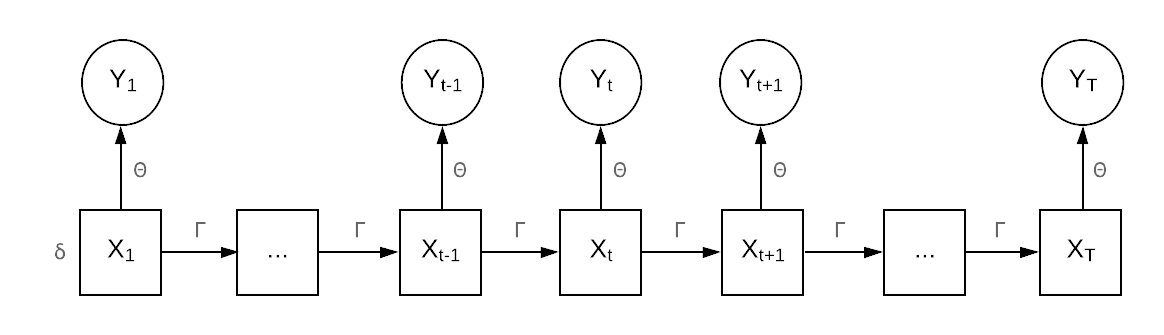
\includegraphics[width=5in]{../Plots/HMM.png}
	\caption{Graphical representation of a traditional HMM.}
	\label{fig:HMM}
\end{figure}


%%%%%%%%%%%%%%%%%%%%%%%%%%%%%%%%%%%%%%%%%
\subsection{The conditionally auto-regressive hidden Markov model (CarHMM)}

A key assumptions of an HMM is \textit{conditional independence} between observations given the state sequence.  Therefore, traditional HMMs do not hold when the observations exhibit certain forms of significant correlation in time.

The CarHMM, or \textit{conditionally auto-regressive hidden Markov model}, introduced by \citep{Lawler:2019}, explicit models auto-correlation within an HMM. Like a traditional HMM, A CarHMM is made up of a Markov chain of unobserved states $X_1,\ldots, X_T$ that can take on values $1, \ldots, N$, with transition probability matrix $\Gamma$ and initial distribution $\delta$ equal to the stationary distribution of $\Gamma$. Unlike a traditional HMM, the CarHMM assumes that the distribution of $Y_t$, conditional on $X_1,\ldots, X_T$ and $ \{Y_1,\ldots, Y_{t-1}\}$, depends on \textit{both} $X_t$ \textit{and} $Y_{t-1}$. 
The first emission $Y_1$ is assumed to be fixed as an initial value which does not depend upon $X_1$. (Fig \ref{fig:CarHMM}) shows the structure of a CarHMM.

\begin{figure}[ht]
	\centering
	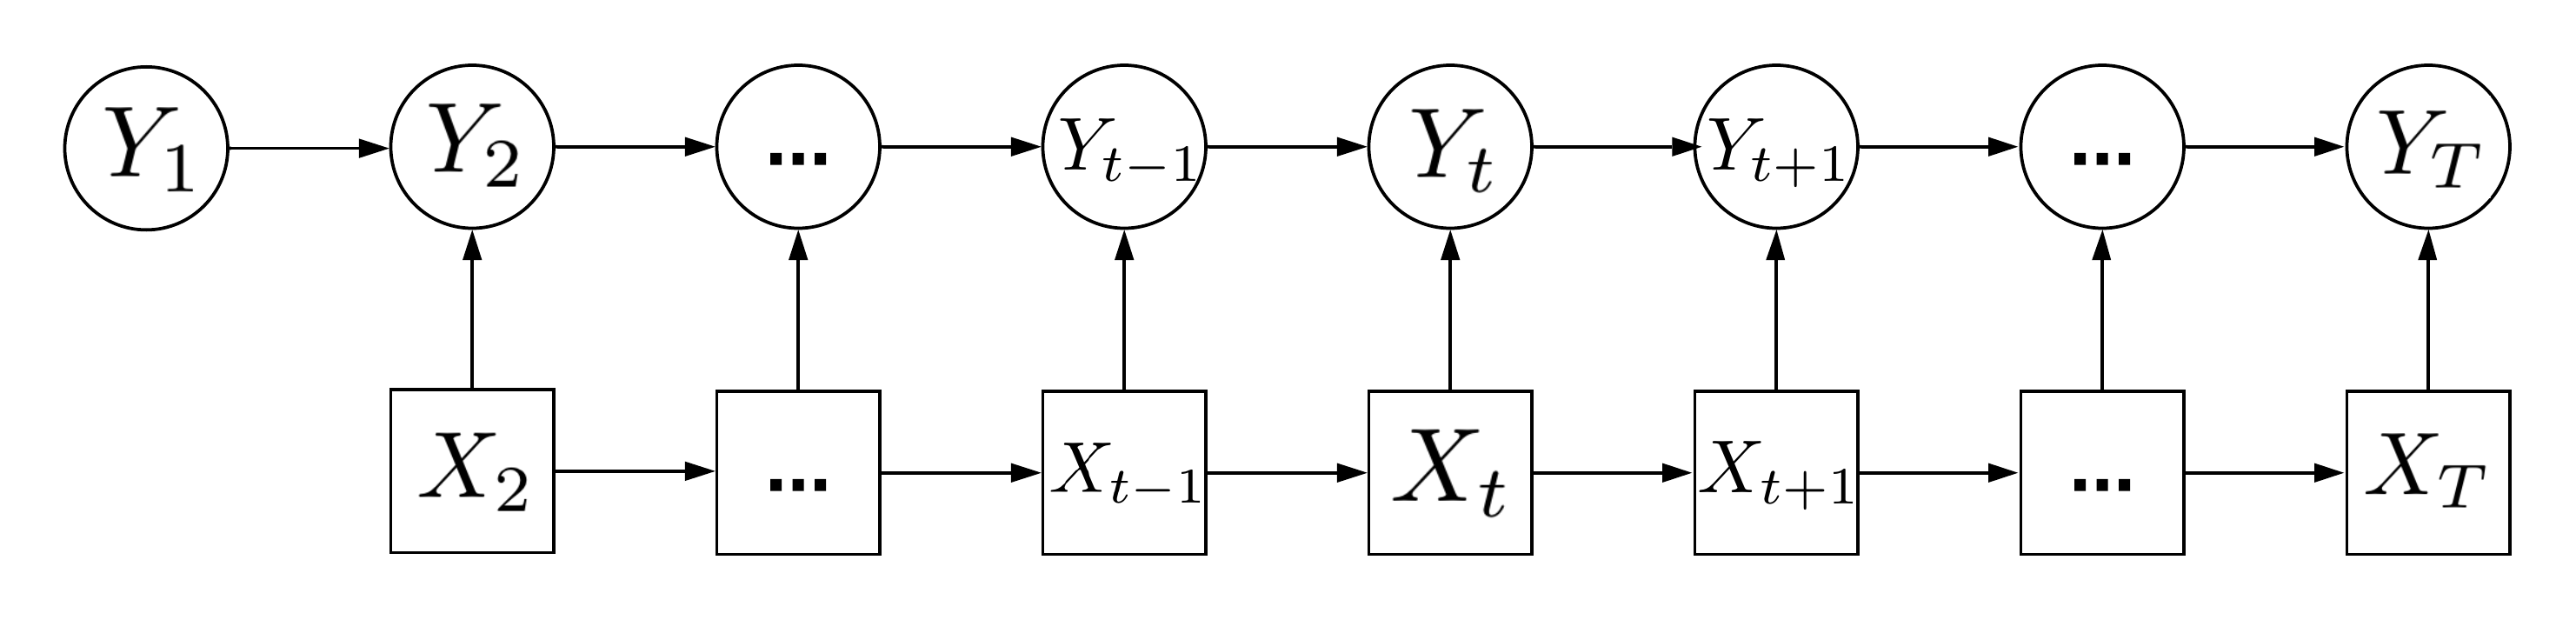
\includegraphics[width=5in]{../Plots/CarHMM.png}
	\caption{Graphical representation of a traditional CarHMM.}
	\label{fig:CarHMM}
\end{figure}

%
We denote the conditional distribution of $Y_t$ given $Y_{t-1}= y_{t-1}$ and $ X_t=i$ as $f^{(i)}( \cdot | y_{t-1}; \theta^{(i)})$ or simply $f^{(i)}( \cdot | y_{t-1})$.
As an example, we could assume that this conditional distribution is normal with parameters $\theta^{(i)} = \{\mu^{(i)},\sigma^{(i)},\phi^{(i)}\}$ where:
%
\[
\mathbb{E}(Y_t|Y_{t-1} = y_{t-1},X_t=i) = \phi^{(i)} ~ y_{t-1} ~+ ~(1-\phi^{(i)})  ~\mu^{(i)}
\]
and
\[
\mathbb{V}(Y_t| Y_{t-1} =y_{t-1}, X_t = i) = (\sigma^{(i)})^2.
\]
%
The likelihood for the CarHMM can be easily calculated using the forward algorithm. As previously, let $y$ be the vector of observed emissions. Then
\begin{equation}
\calL_{\text{CarHMM}}(y;\Theta,\Gamma) = \delta \prod_{t=2}^T \Gamma P(y_t|y_{t-1};\Theta) \mathbf{1}_N
\label{CarHMM_likelihood}
\end{equation}
where
%
$P(y_t|y_{t-1};\Theta)$ is an $N \times N$ diagonal matrix with $ii$th entry equal to $f^{(i)}(y_t|y_{t-1}; \theta^{(i)})$.
%
\subsubsection{Equivalence with continuous-time process}

Although the CarHMM can incorporate auto-correlation into the structure of an HMM, they break down when observations are taken at irregular time intervals since the probability transition matrix $\Gamma$ would then have to depend upon the time step between observations. A common solution to this issue is to use a continuous-time method such as the one introduced by Michelot et al \citep{Michelot:2019}, which models the movement of an animal as an Ornstein-Uhlenbeck process with parameters that depend upon the underlying behavioural state of the animal. Namely, a state-switching Ornstein-Uhlenbeck process $Y$ is the solution to the following stochastic differential equation:
%
\begin{equation}
    \label{eqn:SDE}
    dY_t = \beta^{(X_t)}(\gamma^{(X_t)} - Y_t)dt + \omega^{(X_t)} dW_t
\end{equation}
%
where $X_t$ follows some stochastic process which defines the hidden behaviour of the animal at time $t$, $\beta^{(X_t)}$ relates to rate at which the process returns to its mean value, $\gamma^{(X_t)}$ is the long-term mean value of the process, $\omega^{(X_t)}$ is related to short-term variance, and $W$ is a Wiener process. One notable difference between the state-switching OU process and the CarHMM is that the time index $t \in \mathbb{R}$ exists in continuous time and is not necessarily an integer. If the behavioral state $X_t$ is known and does not change between observations, the solution to (eqn \ref{eqn:SDE}) is known to be the following \citep{Michelot:2019}:
%
\begin{align}
Y_{t+\Delta t} | X_{t} \sim \mathcal{N}\left((1-e^{-\beta^{(X_t)}\Delta t})\gamma^{(X_t)} + e^{-\beta^{(X_t)}\Delta t} Y_t,\quad \frac{\omega^{(X_t)^2}}{2\beta^{(X_t)}} (1-e^{-2\beta^{(X_t)}\Delta t})\right)
\label{eqn:OU_sol}
\end{align}
%
where $\Delta t$ is the time difference between any two observations $Y_t$ and $Y_{t+\Delta t}$. Continuous time models can be built up from arbitrarily complex stochastic differential equations and allow for uneven step lengths in the observations sequence $Y$. However, most continuous time models require MCMC algorithms to perform inference and as a result are not easily incorporated into the HHMM structure.

Although most continuous time models are difficult to incorporate into an HHMM, we show in that under certain conditions, the CarHMM is equivalent to a state-switching Ornstein-Uhlenbeck process shown in (eqn \ref{eqn:OU_sol}). This gives new interpretation to the learned parameters of the CarHMM in the context of a continuous-time model.

\begin{theorem}{Theorem 1.}{}%
If:
\begin{enumerate}
    \item The hidden behavioural process $X$ from (Eq. \ref{eqn:SDE}) follows a Markov chain with $N$ possible states and transitions occur at equi-spaced time stamps $\left(\Delta t, \ldots, (T-1)\Delta t\right)$, and:
    \item Observations of the SDE from (Eq. \ref{eqn:SDE}) are taken at times $\left(0, \Delta t, \ldots, (T-1)\Delta t\right)$,
\end{enumerate}
then the observations $y$ are equivalent to the output of a conditionally auto-regressive hidden Markov model with normal emission distributions and parameters $\Theta = (\theta^{(1)}, \ldots, \theta^{(N)}); \enspace \theta^{(i)} = \{\mu^{(i)},\sigma^{(i)},\phi^{(i)}\}$, where:

\begin{align}
\mu^{(i)} = \gamma^{(i)}, \qquad \sigma^{(i)} = \sqrt{\frac{\omega^{(i)^2}}{2\beta^{(i)}} (1-e^{-2\beta^{(i)}\Delta t})}, \qquad \phi^{(i)} = e^{-\beta^{(i)}\Delta t} \label{eqn:CarHMM_to_OU}
\end{align}

\end{theorem}

See the appendix for a proof of Theorem 1.

\subsection{The hierarchical hidden Markov model (HHMM)}

A \textit{hierarchical hidden Markov model} contains both a coarse-scale process and a fine-scale process, both of which are modeled by an HMM. The coarse-scale process is a hidden Markov model as defined previously, where $X_1, \ldots, X_T$ make up an unobserved Markov chain and $Y_1,\ldots, Y_T$ are the corresponding observed responses. The possible states are $1,\ldots, N$.   
%
In the hierarchical setting, each state $X_t$ emits not only $Y_t$ but also another sequence of fine-scale unobserved states, $X_t^* \equiv (X_{t,1}^*,\ldots, X_{t,T_t^*})$ and a sequence of fine-scale observed emissions, $Y_t^* \equiv (Y_{t,1}^*,\ldots, Y_{t,T_t^*})$. The length of each fine-scale process, $T^*_t$, is a problem-specific tuning parameter. Conditional on the coarse-scale hidden state $X_t$, the joint fine-scale process, ($X_t^*, Y_t^*$), is a hidden Markov model with parameters depending on the value of $X_t$.  Specifically, given that $X_t=i$, $X_t^*$ is a Markov chain with states $1,\ldots, N_t^*$. The distribution of $X_t^*$, conditional on $X_t=i$, is given by an $N^*_t \times N^*_t$ transition probability matrix $\Gamma^{*(i)}$ and initial probability, denoted by the $N_t^*$-vector $\delta^{*(i)}$, which we assume is equal to the stationary distribution of the chain. For simplicity, we take $N_t^* \equiv N^*$ although this is not necessary.
%
The distribution of $Y_{t, t^*}$ given $X_{t, t^*}=i^*$ and $X_t=i$ is governed by a parameter $\theta^{(i,i^*)}$, and has density or probability mass function denoted $f^{*(i,i^*)}\left(\cdot; \theta^{(i,i^*)}\right)$ or sometimes simply denoted by $f^{*(i,i^*)}(\cdot)$. Let $\Theta^{*(i)}=\left(\theta^{(i,1)}, \ldots, \theta^{(i,N^*)}\right)$, the fine-scale emission parameter vector corresponding to $X_t=i$.
%
In terms of the dependence structure, given the coarse-scale states, $X_1,\ldots, X_T$, the $T$ fine-scale processes $(X_1^*, Y_1^*), \ldots, (X_T^*, Y_T^*)$, are independent HMMs. Depending upon the process being modeled, it is possible to force certain parameters to be shared across different coarse or fine states. For example, in the killer whale case study in section \ref{sec:case_study} we force the fine-scale emission parameters to be shared across coarse-scale hidden states, i.e. $\theta^{(1,i^*)} = \ldots = \theta^{(N,i^*)}$ for $i^* = 1, \ldots, N^*$. (Fig \ref{fig:HHMM}) shows the dependence structure for an HHMM.

Due to the nested structure of the hierarchical hidden Markov model, the likelihood remains easy to calculate via the forward algorithm.
%
Let $y$ be the $T$-vector of the observed coarse-scale emissions and
$y^*$ be the $(T_1^* + \cdots T_T^*)$-vector of the observed fine-scale emissions.
%
Let $\Theta^*$ denote the collection of all fine-scale emission parameters,
$\Theta^{*(i)}$, $i=1,\ldots, N$, and let $\Gamma^*$ denote the collection of all fine-scale transition probability matrices, $\Gamma^{*(i)}$, $i=1,\ldots, N$.
%
Then the likelihood of the observed data is
%
\[
\calL_{\text{HHMM}}(y,y^*;\Theta,\Theta^*,\Gamma,\Gamma^*) = \delta P(y_1,y_1^*;\Theta,\Theta^*,\Gamma^*) \prod_{t=2}^T \Gamma P(y_t,y_t^*;\Theta,\Theta^*,\Gamma^*) \mathbf{1}_N
\]
%
where $P(y_t,y_t^*;\Theta,\Theta^*,\Gamma^*)$ is an $N \times N$ diagonal matrix with $ii$th entry corresponding to $X_t=i$ and equal to 
$f^{(i)}(y_t)\calL_{\text{HMM}}\left(y_t^*;\Theta^{*(i)},
\Gamma^{*(i)}\right)$. 

For more information on specific considerations for HHMMs such as incorporating covariates into the probability transition matrix, state decoding, model selection and model checking, see \citep{Adam:2019}.

\begin{figure}[ht]
	\centering
	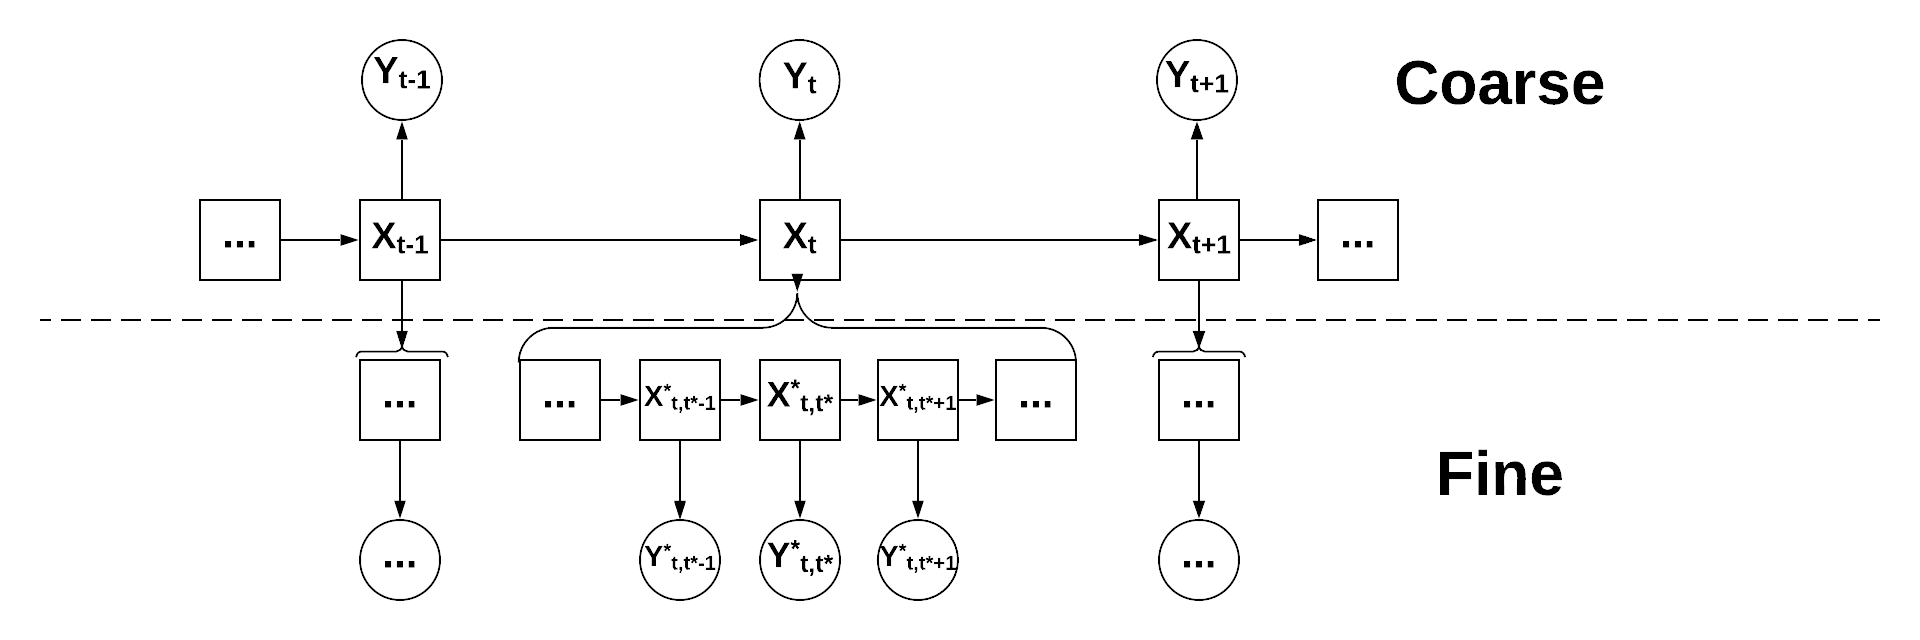
\includegraphics[width=5in]{../Plots/HHMM.png}
	\caption{Graphical representation of a traditional HHMM.}
	\label{fig:HHMM}
\end{figure}



%%%%%%%%%%%%%%%%%%%%%%%%%%%%%%%%%%%%%%%%%
\subsection{The HMM with discrete Fourier transform (HMM-DFT)}
\label{subsec:STFT}

The HMM with discrete Fourier transform or HMM-DFT, is a variation of the hierarchical hidden Markov model where the fine-scale process is no longer modeled with an HMM and instead summarized using it Fourier transform. For simplicity of presentation, we assume that the length of the fine-scale processes is constant, i.e. that $T^*_t = T^*$, although this need not be the case in general. Suppose that the fine-scale process $y^*_t$ does not switch states hidden states, but it does exhibit significant periodic behavior which cannot be modeled with a Markov chain. Then, we suggest using the discrete Fourier transform (DFT) on $y^*_t$:
%
\begin{align*}
    DFT\{y^*_t\}(k) := \hat{y}^{*(k)}_{t} = \sum_{t^* = 1}^{T^*} y^*_{t,t^*}\exp\left(-i \frac{2\pi k}{T^*} (t^*-1)\right) \qquad k = 0, 1, \ldots, T^*-1
\end{align*}
%
Summary statistics can then drastically reduce the dimension of $\hat{y}^*_t$. One example of summary statistics include the following:
%
\begin{equation}
    \label{eqn:z}
    z_t^{*(1)} := \mathcal{R}\left(\hat{y}^{(0)}_t\right) \qquad z_t^{*(2)} := \frac{1}{T^*}\sum_{k=1}^{\tilde{\omega}}|\hat{y}^{(k)}_t|^2
\end{equation}
%
$z_t^{*(1)}$ is equal to the average value of $y^*_t$ and $z_t^{*(2)}$ is equal to the squared 2-norm of the component of $y^*_t$ that can be attributed to frequencies between $1$ and $\tilde{\omega}$ periods per window length $T^*$. The maximum frequency $\tilde{\omega}$ is a problem-specific tuning parameter which should be selected with care. These summary statistics are just one possible choice to describe each window; other choices include the dominant frequency and amplitude of $y^*_t$. Figure (\ref{fig:fourier_example}) visually displays the process of transforming $y^*$ into $z^*$.

\begin{figure}[t]
	\centering
	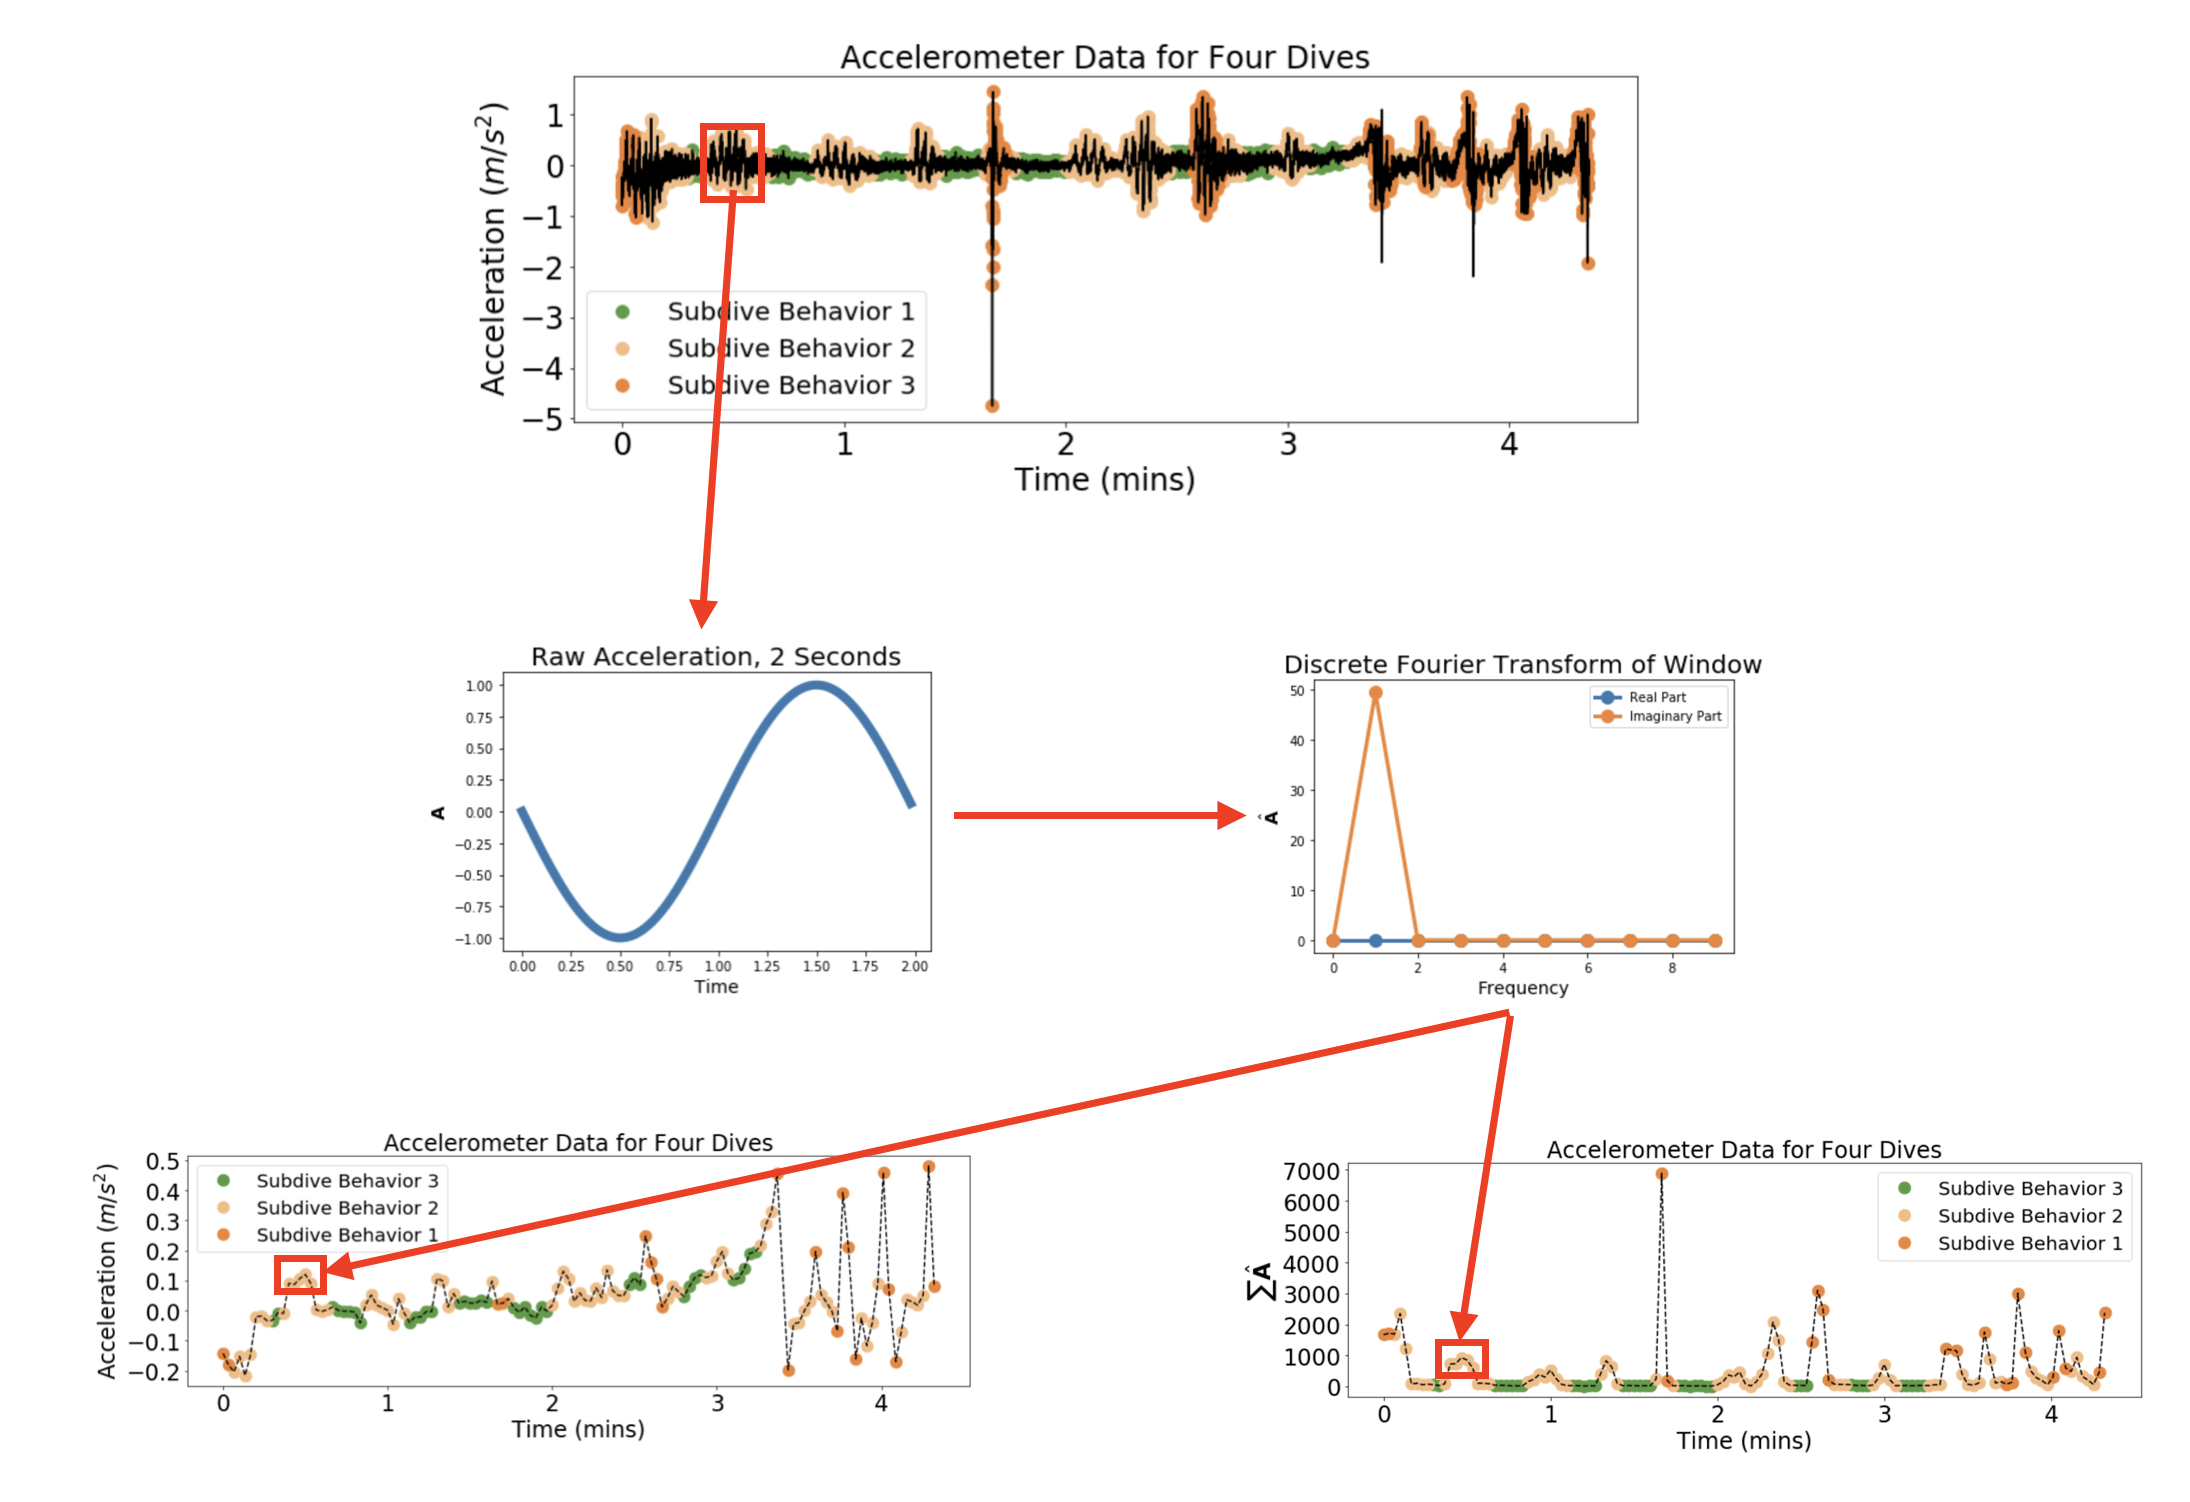
\includegraphics[width=5in]{../Plots/fourier_transform.png}
	\caption{Visualization of transforming $\mathbf{y^*}_t$ into $\mathbf{z}_t$ using a discrete Fourier transform.}
	\label{fig:fourier_example}
\end{figure}

Once $z^*_t$ is calculated, it can simply be treated as an observation of the coarse-scale HMM and incorporated into the emission distribution $f^{(i)}\left(y_t,z^*_t;\theta^{(i)}\right)$, or simply $f^{(i)}\left(y_t,z^*_t\right)$. In total, the likelihood of the hierarchical HMM-DFT is as follows:
\begin{equation}
\calL_{\text{HMM-DFT}}(y,z^*;\Theta,\Gamma) = \delta P(y_1,z^*_1;\Theta) \prod_{t=2}^T \Gamma P(y_t,z^*_t;\Theta) \mathbf{1}_N
\label{HMMDFT_likelihood}
\end{equation}
where $P(y_t,z^*_t;\Theta)$ is an $N \times N$ diagonal matrix with $ii$th entry equal to $f^{(i)}\left(y_t,z^*_t;\theta^{(i)}\right)$.

It is possible to accommodate for unequal time steps within $y_t^*$ by using the non-uniform discrete Fourier transform (NDFT). We do not describe this method here, but the generalization is straightforward. Refer to \citep{Bagchi:1999} for details.

\subsection{General hierarchical structures}

In addition to the DFT and HMM models described above, the fine-scale process $Y^*_t$ can be modeled with \textbf{any} parametric model which admits an easy-to-compute likelihood. The state-specific emission distribution $\calL_{\text{HMM}}$ from the HHMM likelihood is then replaced by the likelihood of the fine-scale model, $\calL_{\text{fine}}(\mathbf{y}^*_t;\Theta^{*(i)})$:
\[
\calL_{\text{coarse}}(y,y^*;\Theta,\Theta^*,\Gamma) = \delta P(y_1,y^*_1;\Theta,\Theta^*) \prod_{t=2}^T \Gamma P(y_t,y^*_t;\Theta,\Theta^*) \mathbf{1}_N
\]
where $P(y_t,y^*_t;\Theta,\Theta^*) $ is an $N \times N$ diagonal matrix with $ii$th entry corresponding to $X_t=i$ and equal to $f^{(i)}\left(y_t;\Theta^{(i)}\right)\calL_{\text{fine}}\left(y^*_t;\Theta^{*(i)}\right)$. This definition is straightforward to extend to the CarHMM as well:
\[
\calL_{\text{coarse}}(y,y^*;\Theta,\Theta^*,\Gamma) = \delta \prod_{t=2}^T \Gamma P(y_t,y^*_t|y_{t-1};\Theta,\Theta^*) \mathbf{1}_N
\]
where $P(y_t,y^*_t|y_{t-1};\Theta,\Theta^*) $ is an $N \times N$ diagonal matrix with $ii$th entry corresponding to $X_t=i$ and equal to $f^{(i)}\left(y_t|y_{t-1};\Theta^{(i)}\right)\calL_{\text{fine}}\left(y^*_t;\Theta^{*(i)}\right)$

As previously mentioned, the fine-scale model can be any parametric model with easy-to-compute likelihood, including any of the four models described in the previous four subsections (HMM, CarHMM, HHMM, and HMM-DFT). These HMM models then act as building blocks that can be used to build increasingly complex hierarchical models based on the HMMs. In the sections that follow, we perform both a simulation study and real-world case study modelling killer whale dive behaviour using models built from these building blocks.